\documentclass{beamer}
\title{Reed-Muller Error-Correcting Codes}
\author{Prateek Sharma}
\date{April 30, 2010}
\usetheme[]{Warsaw}
%\usefonttheme{serif}
\usecolortheme{seahorse}
%\usecolortheme{rose}
\includegraphics{}

\newcommand{\RM}[2]{\ensuremath{\mathcal{R}(#1,#2)}}

\newcommand{\rem}{Reed-Muller}

\newcommand{\F}{\ensuremath{\mathbb{F}}}

\newcommand{\V}[1]{\ensuremath{\mathbf{#1}}}

\newcommand{\slm}{Sloane MacWilliams}

\begin{document}
\maketitle

%%%%%%%%%%%%%%%%%%%%%%%%%%%%%%%%%%%%%%%%%%%%%%%%%%%%%%%%


\begin{frame}
 \frametitle{Reed-Muller codes}
\begin{}
The Reed-Muller codes are a family of error-correcting codes. They are
the oldest known codes after the Hamming and the Golay codes.
\end{}

\begin{itemize}
In this talk:
\item Code properties: Distance, dimension, orthogonal code
\item Decoding Algorithms 
\item Applications of \rem{} codes
\end{itemize}

Most famously used in the Mariner-9 spacecraft in 1972 to transmit clear images of the martian surface.
\end{frame}


%%%%%%%%%%%%%%%%%%%%%%%%%%%%%%%%%%%%%%%%%%%%%%%%%%%%%%%%%%%

\begin{frame}{Mariner-9}
\begin{figure}
   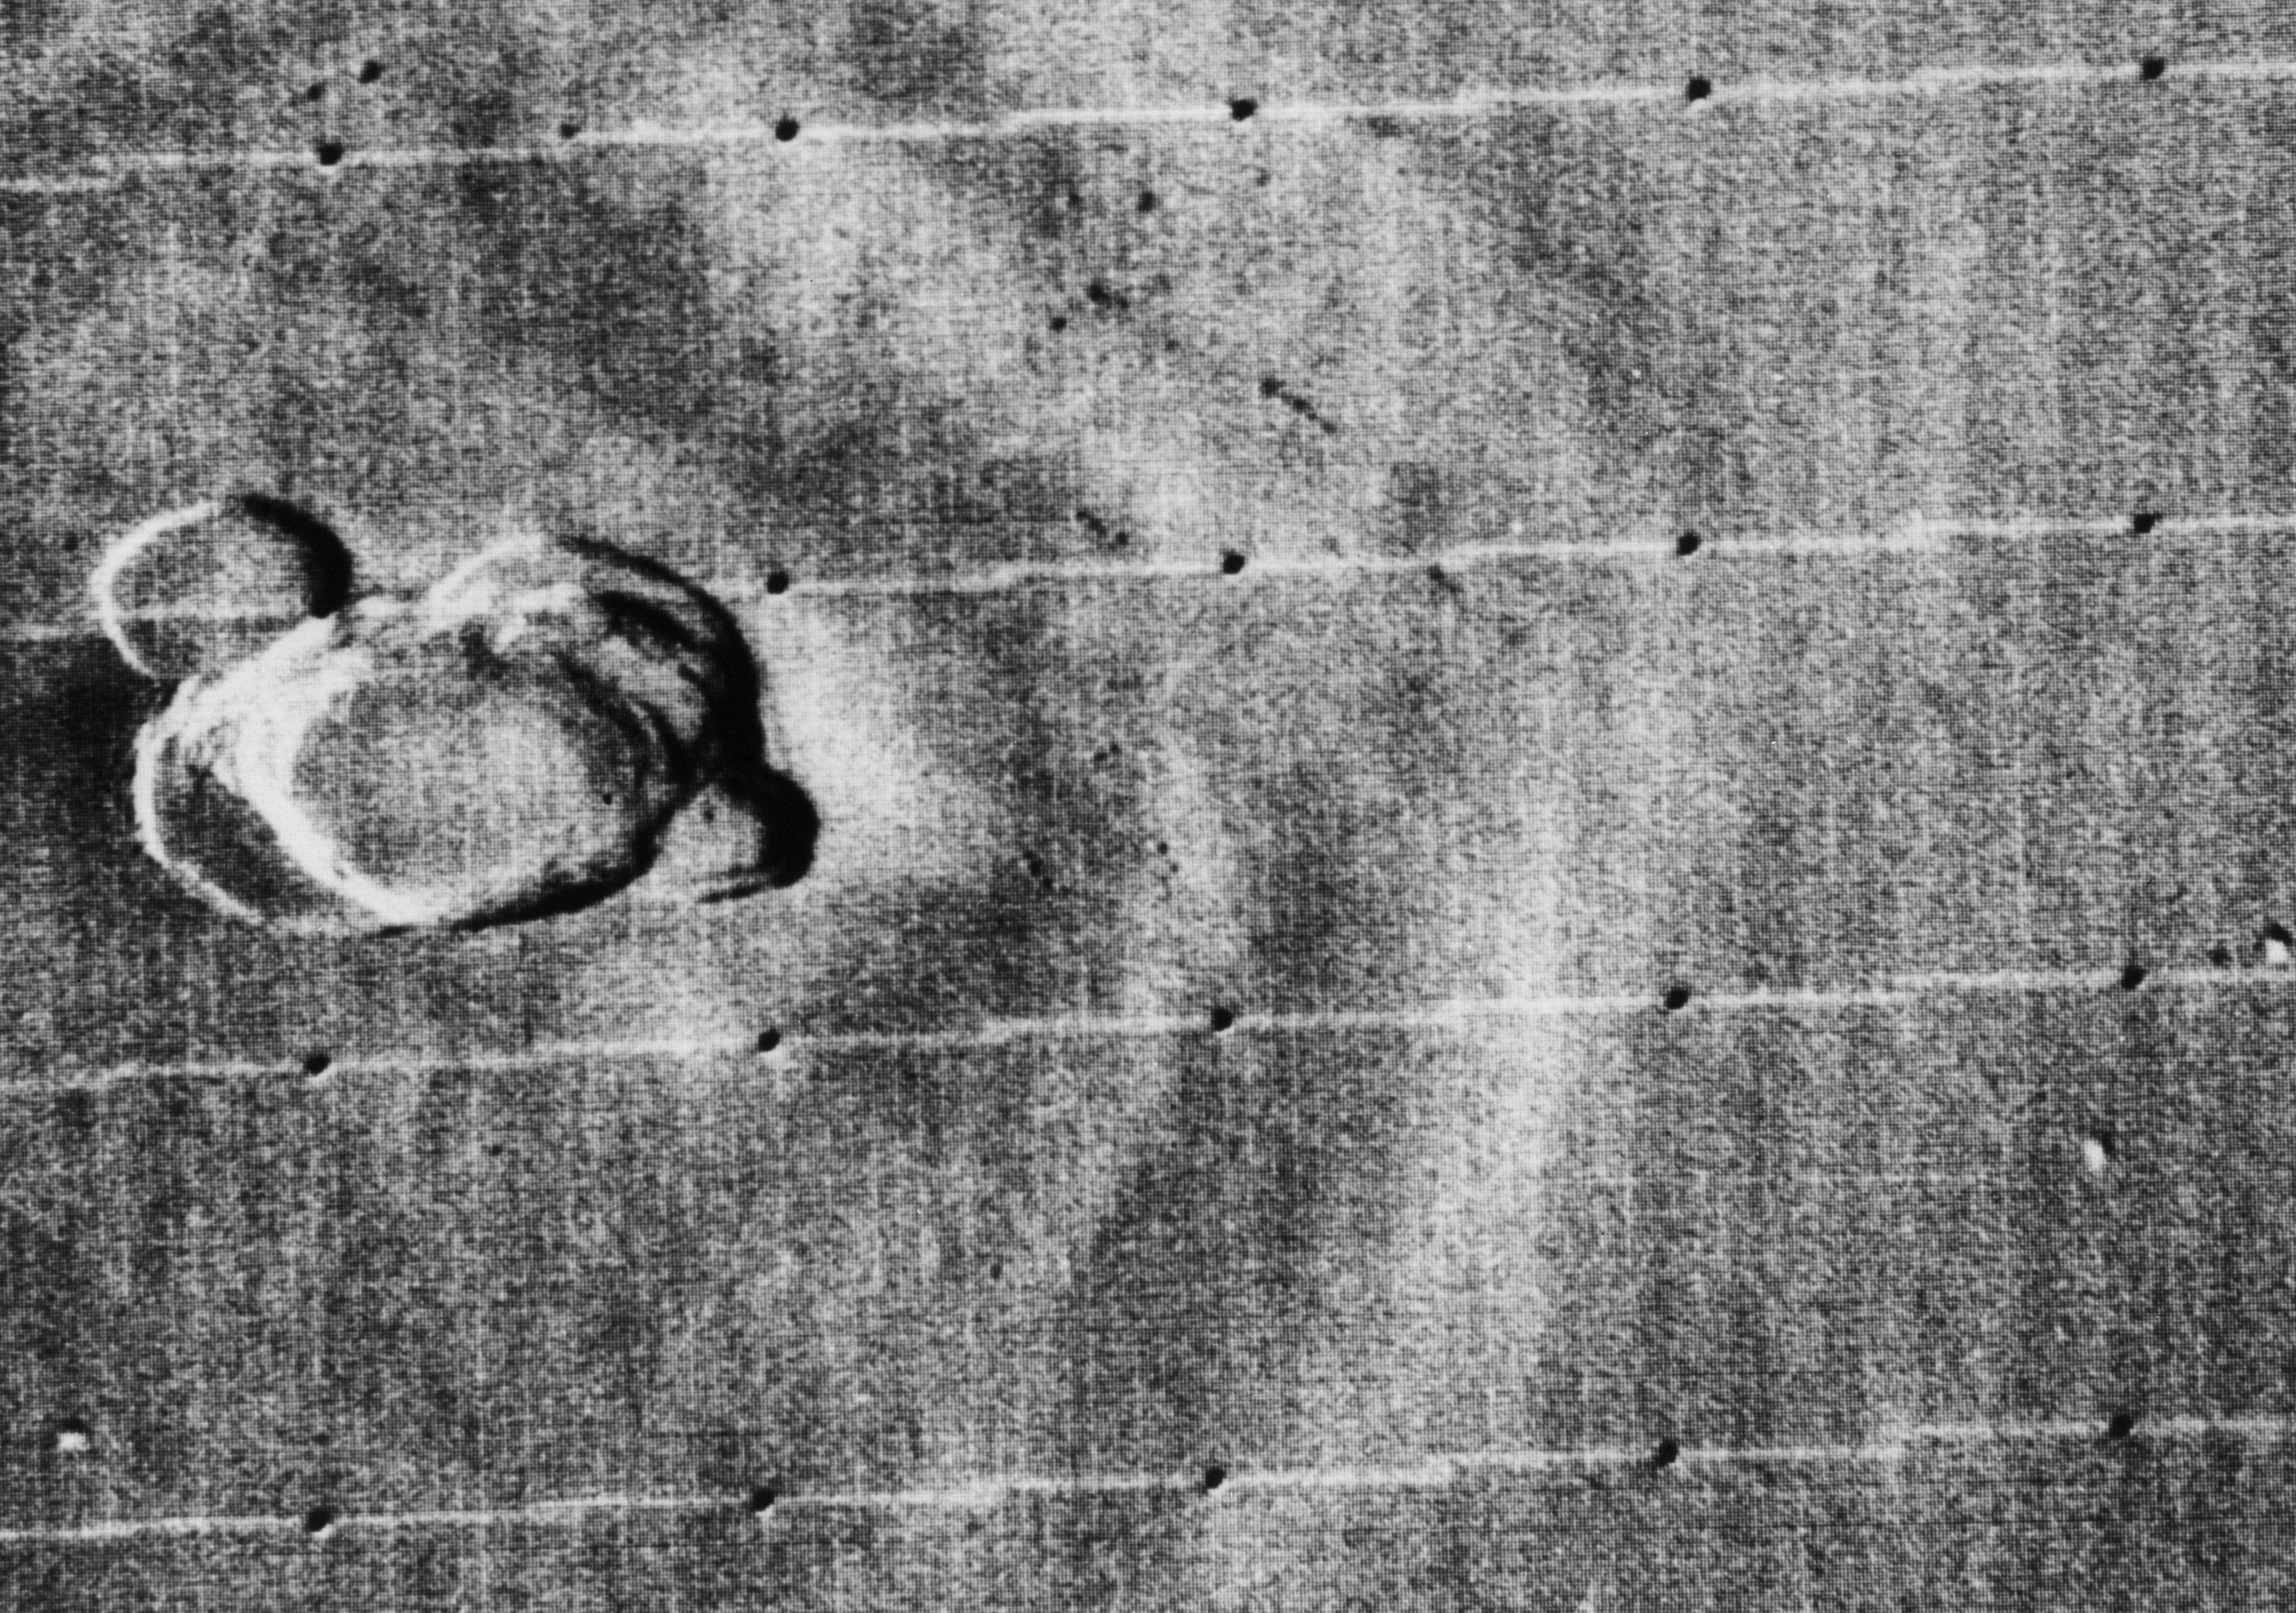
\includegraphics[scale=0.10]{mariner9.jpg}
\end{figure}

\end{frame}

%%%%%%%%%%%%%%%%%%%%%%%%%%%%%%%%%%%%%%%%%%%%%%%%%%%%%%%%


\begin{frame}

\frametitle{Construction}
$\V{x} \equiv (x_1,x_2,\ldots,x_m) \in \F^m$
\newline

\begin {center}
\begin{tabular}{|c|c|c|c|c|c|c|c|c|}
\hline
$x_1$ & $0$ & $0$ & $0$ & $0$ & $1$ & $1$ & $1$ & $1$ \\
$x_2$ & $0$ & $0$ & $1$ & $1$ & $0$ & $0$ & $1$ & $1$ \\
$x_3$ & $0$ & $1$ & $0$ & $1$ & $0$ & $1$ & $0$ & $1$ \\
\hline
$f$   & $0$ & $1$ & $0$ & $1$ & $0$ & $1$ & $1$ & $0$ \\
\hline
\end{tabular}
\end{center} 

Disjunctive Normal Form
$f = x_3 + x_1x_2$.

$(x_1,x_2,\ldots,x_m)$ can take $2^m$ values, $\V{f}$ is a $n=2^m$
length vector over $F_2$.
$2^{2^m}$ such Boolean functions possible, giving a collection of  $2^{2^m}$ vectors, each of length $2^m$.

\end{frame}

%%%%%%%%%%%%%%%%%%%%%%%%%%%%%%%%%%%%%%%%%%%%%%%%%%%%%%%%


\begin{frame}
 \frametitle{Boolean Monomials}
\begin{equation*}
M = \{1,x_1,x_2,\ldots,x_m,x_1x_2,\ldots,x_{m-1}x_m,x_1x_2x_3,\ldots,x_1x_2\ldots x_m\}
\end{equation*}

\begin{equation*}
  f = 1 + a_1x_1+a_2x_2+\ldots+a_mx_m + a_{12}x_1x_2+\ldots+a_{12\ldots r}x_1x_2\ldots x_r+\ldots
\end{equation*}

Since $\V{f}$ is a linear combination, it follows that the length of $x_1, x_2,\ldots,x_m$ is $2^m$.

\begin{equation*}
  1+\binom{m}{1}+\binom{m}{2}+\ldots+\binom{m}{m} = 2^m 
\end{equation*}
\end{frame}

%%%%%%%%%%%%%%%%%%%%%%%%%%%%%%%%%%%%%%%%%%%%%%%%%%%%%%%%


\begin{frame}
 \frametitle{First-order codes}

\begin{defn}
The \rem{} codes of order $r$ and length $n = 2^m$ ,$0 \leq r \leq m$  is the set of all vectors $\V{f}$, where $f(x_1,\ldots,x_m)$ is a Boolean function which is a polynomial of degree at most $r$.
\end{defn}


\begin{equation}
 \V{1}+a_1\V{x_1}+a_2\V{x_2}+\ldots+a_m\V{x_m}
\end{equation}


\end{frame}

%%%%%%%%%%%%%%%%%%%%%%%%%%%%%%%%%%%%%%%%%%%%%%%%%%%%%%%%

\begin{frame}
 \frametitle{Linearity}
\begin{Lemma}[Linearity]
  $\RM{r}{m}$ is a linear code.
\end{Lemma}

\begin{obs}
  The monomials of degree $\leq r$ form a basis for $\RM{r}{m}$.
\end{obs}

Generator matrix
\begin{equation}
  \label{eq:5}
  G(r,m) =
  \begin{pmatrix}
    \V{1} \\
    \V{x_1} \\
    \V{x_2} \\
    \vdots \\
    \V{x_m} \\
    \V{x_1x_2} \\
    \vdots \\
    \V{x_1x_2\ldots x_r}
  \end{pmatrix}
\end{equation}

\end{frame}

%%%%%%%%%%%%%%%%%%%%%%%%%%%%%%%%%%%%%%%%%%%%%%%%%%%%%%%%

\begin{frame}
 \begin{obs}
  The dimension ($k$) of $\RM{r}{m}$ is equal to the  number of monomials of degree $\leq r$.
\end{obs}

\begin{equation}
  \label{eq:2}
 k= 1+\binom{m}{1}+\binom{m}{2}+\ldots+\binom{m}{r}
\end{equation}

From what we have seen so far, we observe that $\RM{0}{m} $ is the repetition code ($2^m$ repetition). At the other extreme $\RM{m}{m}$ is a code consisting of all possible binary sequences of length $2^m$.

A summary of the properties of $\RM{r}{m}$ :
\begin{center}
\begin{tabular}[center]{|c|c|}
\hline
Length & $n = 2^m$ \\
Minimum Distance & $d = 2^{m-r}$ \\
Dimension & $k= 1+\binom{m}{1}+\binom{m}{2}+\ldots+\binom{m}{r}$ \\
\hline
\end{tabular}
\end{center}

Thus, $\RM{r}{m}$ is an $[2^m,1+\binom{m}{1}+\binom{m}{2}+\ldots+\binom{m}{r}, 2^{m-r}]$ linear code.

\end{frame}

%%%%%%%%%%%%%%%%%%%%%%%%%%%%%%%%%%%%%%%%%%%%%%%%%%%%%%%%%%%%%

\begin{frame}
 \begin{equation}

\RM{1}{3} = \begin{array}{|l|cccccccc|}
  position &     0&1&2&3&4&5&6&7 \\
\hline
1 \quad&  	 1&1&1&1&1&1&1&1 \\
x_1 \quad& 	 0&0&0&0&1&1&1&1 \\
x_2 \quad& 	 0&0&1&1&0&0&1&1 \\
x_3 \quad&	 0&1&0&1&0&1&0&1 \\
x_1+x_2 \quad&    0&0&1&1&1&1&0&0 \\
x_1+x_3 \quad&	 0&1&1&0&0&1&1&0 \\
x_2+x_3 \quad&	 0&1&0&1&1&0&1&0 \\
x_1+x_2+x_3 \quad& 0&1&1&0&1&0&0&1 \\
1+x_1	\quad&	 1&1&1&1&0&0&0&0 \\
1+x_2	\quad&	 1&1&0&0&1&1&0&0 \\
1+x_3	\quad&	 1&0&1&0&1&0&1&0 \\
1+x_1+x_2 \quad&	 1&1&0&0&0&0&1&1 \\
1+x_1+x_3 \quad&	 1&0&0&1&1&0&0&1 \\
1+x_2+x_3 \quad&	 1&0&1&0&0&1&0&1 \\
1+x_1+x_2+x_3\quad& 1&0&0&1&0&1&1&0 \\
\hline
\end{array}
\end{equation}
\end{frame}

%%%%%%%%%%%%%%%%%%%%%%%%%%%%%%%%%%%%%%%%%%%%%%%%%%%%%%%%%%%%%%

\begin{frame}
 \begin{equation}
G(2,3) =\begin{array}{|l|cccccccc|}
\hline
1 \quad&         1&1&1&1&1&1&1&1 \\
x_1 \quad&       0&0&0&0&1&1&1&1 \\
x_2 \quad&       0&0&1&1&0&0&1&1 \\
x_3 \quad&       0&1&0&1&0&1&0&1 \\
x_1\cdot x_2 \quad& 0&0&0&0&0&0&1&1 \\ 
x1\cdot x_3 \quad& 0&0&0&0&0&1&0&1 \\
x2\cdot x_3 \quad& 0&0&0&1&0&0&0&1 \\
\hline
\end{array}
\end{equation}
\end{frame}

%%%%%%%%%%%%%%%%%%%%%%%%%%%%%%%%%%%%%%%%%%%%%%%%%%%%%%%%%%%%%%

\begin{frame}
 \frametitle{Recursive formulation}
\begin{theorem}
\begin{equation*} \RM{r+1}{m+1} =  \{ \V{u} | \V{u}+\V{v} : \V{u} \in \RM{r+1}{m}, \V{v} \in \RM{r}{m} \} \end{equation*}
\end{theorem}

\begin{equation}
G(r+1,m+1) = \begin{pmatrix}
G(r+1,m) & G(r+1,m) \\
0 & G(r,m) 
\end{pmatrix}
\end{equation}

\begin{equation}
G(1,m+1) = \begin{pmatrix}
G(1,m) & G(1,m) \\
0 & 1
\end{pmatrix}
\end{equation}
where
\begin{equation*}
  G(0,m) = ( {\overbrace{\V{1111}}^{2^m}} )
\end{equation*}


\end{frame}

%%%%%%%%%%%%%%%%%%%%%%%%%%%%%%%%%%%%%%%%%%%%%%%%%%%%%%%%%%%%%%%%%%

\begin{frame}
 \begin{theorem}
\begin{equation*}
\RM{r}{m} \subseteq \RM{t}{m} \quad
\text{ if } 0 \leq r \leq t \leq m \\
\end{equation*}
\end{theorem}

\begin{theorem}
\label{general}
$C_i$ : $[n,k_i,d_i]$ code. The concatenated code

  \begin{equation*}
    C = \{(\V{u},\V{u}+\V{v}) | \V{u} \in C_1 , \V{v} \in C_2 \}
  \end{equation*}

has the parameters $[2n,k_1+k_2, min\{2d_1,d_2\}]$ .
\end{theorem}

\begin{obs}
  \label{eq:1}
  \begin{equation*}
      dim(\RM{r}{m}) = dim(\RM{r}{m-1}) + dim(\RM{r-1}{m-1})
  \end{equation*}
\end{obs}

\end{frame}

%%%%%%%%%%%%%%%%%%%%%%%%%%%%%%%%%%%%%%%%%%%%%%%%%%%%%%%%%%%%%%%%

\begin{frame}
 \framtitle{Distance properties}
\begin{theorem}
Minimum distance, $d=2^{m-r}$
\end{theorem}

\begin{obs}
\label{equidistant}
Every codeword in $\RM{1}{m}$ (except $\V{1}, \V{0}$) has weight $2^{m-1}$
\end{obs}

\end{frame}

%%%%%%%%%%%%%%%%%%%%%%%%%%%%%%%%%%%%%%%%%%%%%%%%%%%%%%%%%%%%%%%%

\begin{frame}
\frametitle{Dual and Orthogonal of RM codes}
\begin{theorem}
  \begin{equation*}
    \RM{m-r-1}{m} = \RM{r}{m}^{\bot}
  \end{equation*}
\end{theorem}

\begin{theorem}
The dual code $\RM{1}{m}^{\bot}$ is the extended binary Hamming code $H(m)$ 
\end{theorem}

The \emph{orthogonal code} $\mathcal{O}_m$ to be the $[2^m, m, 2^{m-1}]$ code consisting of the vectors $ \sum_{i=1}^m{u_i\V{v_i}} $

\begin{theorem}
  \begin{equation*}
  \RM{1}{m} = \mathcal{O}_m \cup (\V{1} + \mathcal{O}_m) 
\end{equation*}
\end{theorem}

\end{frame}

%%%%%%%%%%%%%%%%%%%%%%%%%%%%%%%%%%%%%%%%%%%%%%%%%%%%%%%%%%%%%%


\begin{frame}
 \frametitle{uniqueness}
\begin{theorem}
   Any linear code with parameters $[2^m, m+1, 2^{m-1}]$ is equivalent to the first order \rem{} code.
\begin{proof}
[Proof in \cite{uniq}]
\end{proof} \label{uniqness}
\end{theorem}

\end{frame}


%%%%%%%%%%%%%%%%%%%%%%%%%%%%%%%%%%%%%%%%%%%%%%%%%%%%%%%%%%%%%%

\begin{frame}
 \frametitle{Plotkin Bound}

\begin{theorem}[Plotkin Bound]
    If $C = [n,k,d]$ code, \begin{equation*}
d \leq \frac{n2^{k-1}}{2^k - 1}
\end{equation*}
  \begin{proof}
Counting in two ways:
\end{proof}
\end{theorem}


\end{frame}


%%%%%%%%%%%%%%%%%%%%%%%%%%%%%%%%%%%%%%%%%%%%%%%%%%%%%%%%%%%%%%

\begin{frame}
\frametitle{Decoding}
Major decoding approaches for \rem{} codes
Majority logic decoding
Step Decoding
Hadamard Transforms (only for $\RM{1}{m}$)
List Decoding 
\emph{And a lot more soft/hard decoding algorithms}
\end{frame}

%%%%%%%%%%%%%%%%%%%%%%%%%%%%%%%%%%%%%%%%%%%%%%%%%%%%%%%%%%%%%%

\begin{frame}
\frametitle{Majority-Logic Decoding}
Message bit parities voted by multiple bits in the received vector.
 \begin{equation}

\RM{1}{3} = \begin{array}{|l|cccccccc|}
  position &     0&1&2&3&4&5&6&7 \\
\hline
1 \quad&  	 1&1&1&1&1&1&1&1 \\
x_1 \quad& 	 0&0&0&0&1&1&1&1 \\
x_2 \quad& 	 0&0&1&1&0&0&1&1 \\
x_3 \quad&	 0&1&0&1&0&1&0&1 \\
x_1+x_2 \quad&    0&0&1&1&1&1&0&0 \\
x_1+x_3 \quad&	 0&1&1&0&0&1&1&0 \\
x_2+x_3 \quad&	 0&1&0&1&1&0&1&0 \\
x_1+x_2+x_3 \quad& 0&1&1&0&1&0&0&1 \\
1+x_1	\quad&	 1&1&1&1&0&0&0&0 \\
1+x_2	\quad&	 1&1&0&0&1&1&0&0 \\
1+x_3	\quad&	 1&0&1&0&1&0&1&0 \\
1+x_1+x_2 \quad&	 1&1&0&0&0&0&1&1 \\
1+x_1+x_3 \quad&	 1&0&0&1&1&0&0&1 \\
1+x_2+x_3 \quad&	 1&0&1&0&0&1&0&1 \\
1+x_1+x_2+x_3\quad& 1&0&0&1&0&1&1&0 \\
\hline
\end{array}
\end{equation}



\begin{example}
$\V{x} = 00110110 \in \RM{1}{3}$

\end{example}

\end{frame}


%%%%%%%%%%%%%%%%%%%%%%%%%%%%%%%%%%%%%%%%%%%%%%%%%%


\begin{frame}
\frametitle{Orthogonal checksums}
Ideally, want \emph{orthogonal} sums each coordinate.

\begin{equation*}
x_0 + x_1 + x+3 = 0
x_0 + x_4 + x_5 = 0
x_0 + x_2 + x_6 = 0
\end{equation*}
 is orthogonal on $0$ .


\begin{thm} 
$J$ parity checks on every co-ordinate can correct $\lfloor\frac{J}{2}\rfloor$ errors.
\end{thm}

Finding orthogonal checksums is assisted by finite geometries

\begin{thm}
  For $\RM{r}{m}$, $(r+1)$-step majority decoding can correct $\lfloor \frac{1}{2}(d-1) \rfloor$ errors.
  \begin{proof}
    See \slm{} \cite{sloane} Chapter-13 ,Theorem-20 .
  \end{proof}
\end{thm}

\end{frame}





%%%%%%%%%%%%%%%%%%%%%%%%%%%%%%%%%%%%%%%%%%%%%%%%%%

\begin{frame}
\frametitle{Hadamard Transform}


\end{frame}


%%%%%%%%%%%%%%%%%%%%%%%%%%%%%%%%%%%%%%%%%%%%%%%%%%

\begin{frame}
\frametitle{Algorithm} 

\end{frame}

%%%%%%%%%%%%%%%%%%%%%%%%%%%%%%%%%%%%%%%%%%%%%%%%%%


\begin{frame}
\frametitle{Applications} 

\end{frame}

%%%%%%%%%%%%%%%%%%%%%%%%%%%%%%%%%%%%%%%%%%%%%%%%%%

\end{document}
